\section{分析手法}
この節では歌詞印象推定手法で用いた分析手法について紹介する.
\subsection{MAP推定}
MAP推定とは事前知識に基づいて未知のデータを点推定する手法である.
θを尤度,Dを事前知識とすると,ベイズの定理に基づき次の式(3.1)で表せる.
\begin{equation}
\begin{split}
\rm{argmax_{θ}P(θ|D)}&\rm{=argmax_θ\frac{P(D|θ)P(θ)}{P(D)}}\\
&\rm{=argmax_{θ}P(D|θ)P(θ)}
\end{split}
\end{equation}
ここで分母のP(D)は尤度θと関係がないので無視する.P(D\verb+|+θ)は尤度関数,P(θ)は事前分布,P(θ\verb+|+D)は事後分布と呼ぶ.
事前分布P(θ)は複雑な計算を要する.そのため,それを回避するために事前分布の代わりに共役事前分布を用いて推定をする.共役事前分布とは尤度をかけて事後分布を求めるとその関数の形が同じになる事前分布のことである.
事後分布が最大となる尤度θを算出するのがMAP推定である.

本研究ではカテゴリカル分布に基づくMAP推定をする.
したがって事前知識Dはカテゴリカル分布に従うN個の離散値データ$\rm{D=\{d_1,d_2,...d_N\}}$と定義する.
尤度関数はカテゴリカル分布の確立質量関数で表せるので式(3.2)となる.
\begin{equation}
\begin{split}
\rm{P(D|θ)=\prod^N_{n=1}Cat(d_n|θ)}
\end{split}
\end{equation}
カテゴリカル分布の共役事前分布はディリクレ分布であるため事前分布を式(3.3)で表す.ディリクレ分布はハイパーパラメータαが大きくなるにつれて分散が小さくなる特性を持つ.
ハイパーパラメータαは対応する事象dの観測数の初期値を意味する.αを全て1とした場合,ディリクレ分布は一様な無情報事前分布となり,事後分布は尤度関数であるカテゴリカル分布と同じ分布になる.
\begin{equation}
\begin{split}
\rm{P(θ)\propto{Dir(θ;\alpha)}}
\end{split}
\end{equation}
式(3.2)と式(3.3)を式(3.1)に当てはめると事後分布は式(3.4)のように表せる.
\begin{equation}
\begin{split}
\rm{P(θ|D)\propto\{\prod^N_{n=1}Cat(d_n|θ)\}Dir(θ;\alpha)}
\end{split}
\end{equation}
式(3.4)の両辺に対数をとった式(3.5)を示す.ここで$\rm{d_{n,k}}$はK次元ベクトル$\rm{d_n}$のk番目の要素を指し示す.$\mathbb{C}$は不定定数である.
\begin{equation}
\begin{split}
\rm{\log P(θ|D)}&\rm{\propto\sum^N_{n=1}\log Cat(d_n|θ)+\log Dir(θ;\alpha)+\mathbb{C}}\\
&\rm{=\sum^K_{k=1}(\sum^N_{n=1}d_{n,k}+\alpha_{n,k}-1)\log θ_k+\mathbb{C}}
\end{split}
\end{equation}
このまま偏微分しても極値を得ることはできないのでラグランジュの未定乗数法を使用する.ラグランジュ関数は式(3.6)である.
\begin{equation}
\begin{split}
\rm{L=\log P(θ|D)+\lambda(\sum^K_{k=1}θ_k-1)}
\end{split}
\end{equation}
ラグランジュ関数Lを$\rm{θ_k}$で偏微分して0となる極値を求めるとMAP推定値$\rm{{\hat\mu}_{map,k}}$が得られる.
\begin{equation}
\begin{split}
\rm{{\hat\mu}_{map,k}=\frac{\alpha_k-1+θ_k}{1-K+\sum^K_{j=1}\alpha_j}}
\end{split}
\end{equation}
\subsection{PLSA}
PLSA[12]とは次元圧縮手法の一種であり,情報検索の分野で膨大な文書データを分類するために研究された手法である.
PLSAは文書dとその文書中に出現する単語wの間に共通のトピックと呼ぶ潜在意味クラスzが存在することを想定として,潜在意味クラスzを確率的に推定する手法である.
そして,文書dと単語wの共起確率P(d,w)を潜在意味クラスzを用いてモデル化する.zでモデル化したP(d,w)の式を式(3.8)にグラフィカルモデルを図1に示す.
\begin{equation}
\begin{split}
\rm{P(d,w)=\sum_zP(z)P(d|z)P(w|z)}
\end{split}
\end{equation}

\begin{figure}[h]
  \centering
  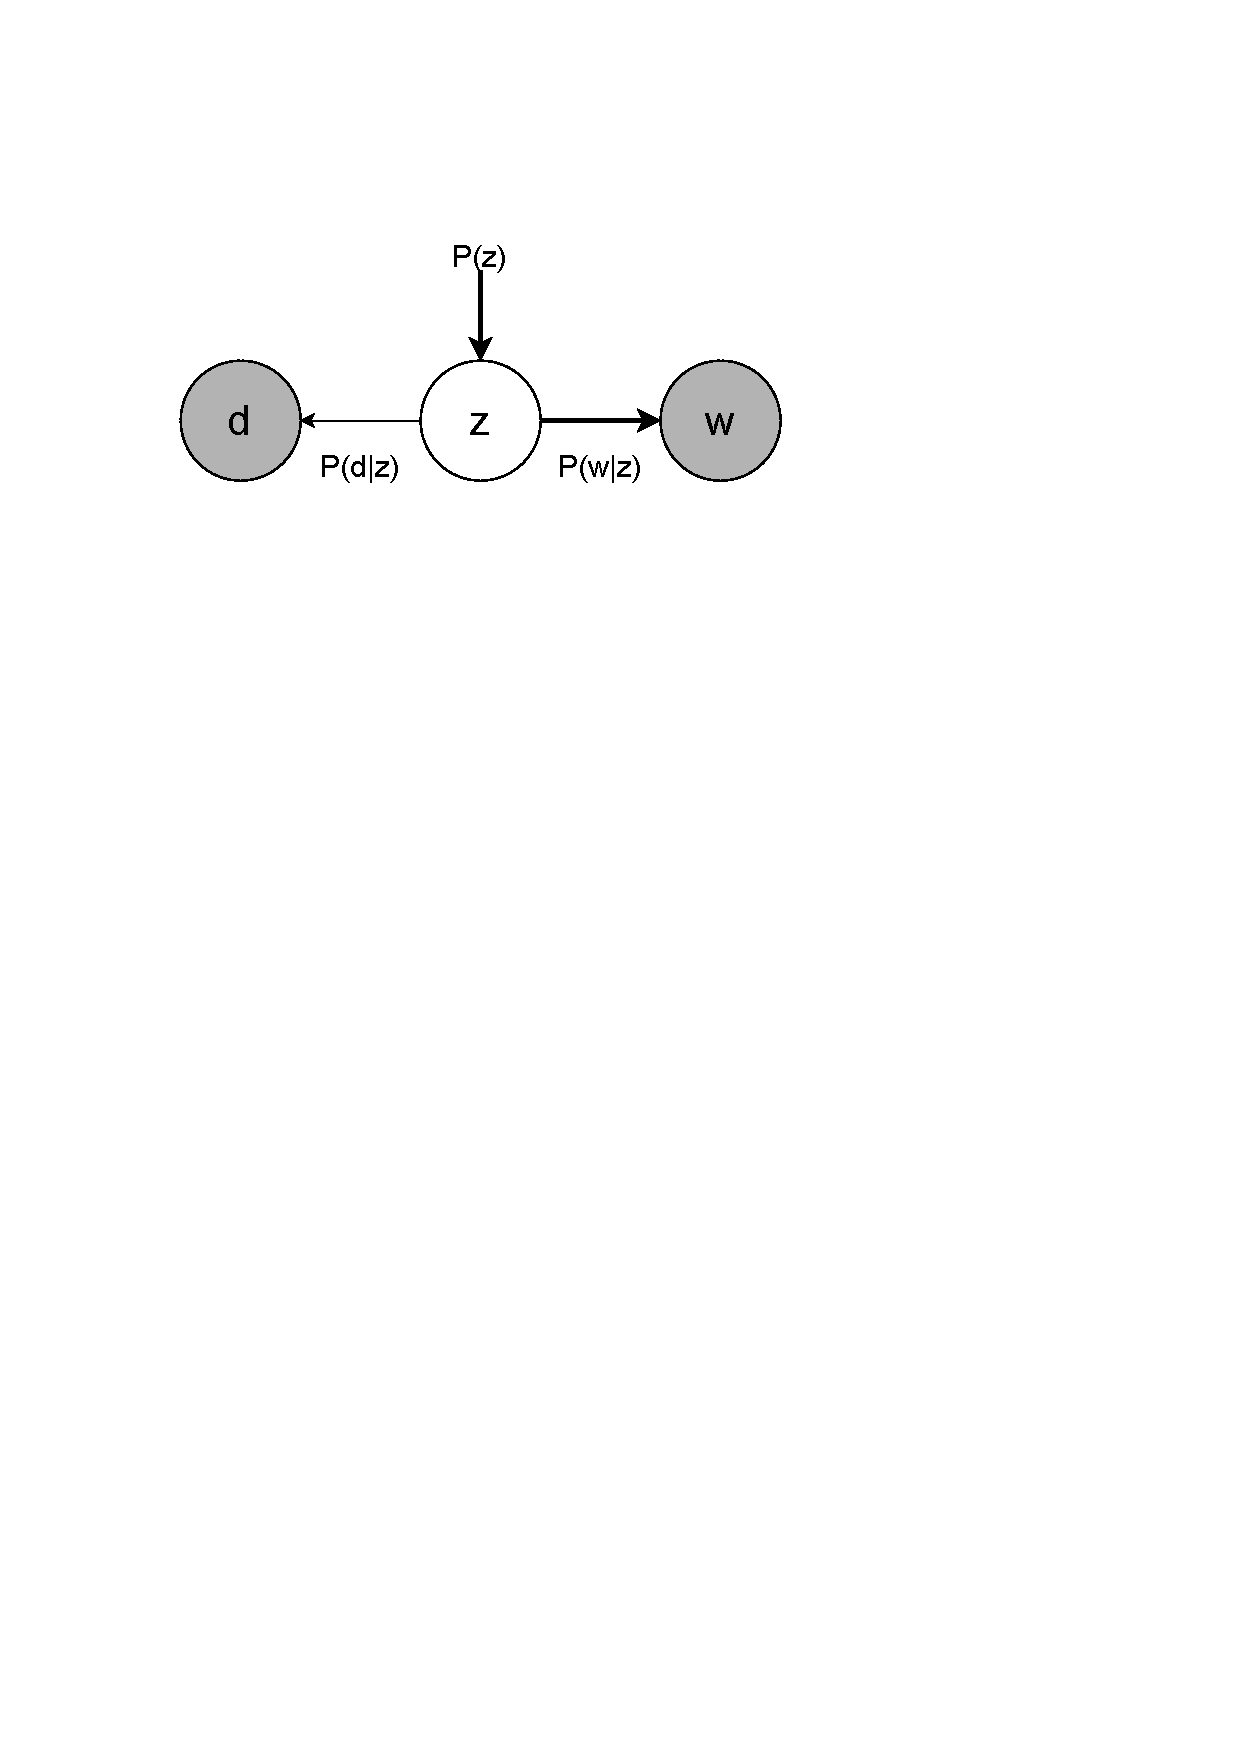
\includegraphics[width=12cm]{PLSA_graphical.pdf}
  \vspace{-1mm}
  \caption{PLSAグラフィカルモデル}
  \label{fig:vkall}
  \vspace{5mm}
\end{figure}
文書dと単語wの同時出現頻度をN(d,w)とすると,対数尤度関数logLは式(3.9)として示せる.
\begin{equation}
\begin{split}
\rm{\log L= \sum_d\sum_wN(d,w)\log(P(d,w))}
\end{split}
\end{equation}
この対数尤度関数logLを最大にする確率変数P(z),P(d\verb+|+z),P(w\verb+|+z)をEMアルゴリズムによって推定する.なお推定する確率変数をモデルパラメータと呼ぶ.EMアルゴリズムとは混合分布モデルのパラメータ推定に利用できる学習アルゴリズムである.
zの確率分布P(z\verb+|+d,w)を予測するE(expectation)ステップと対数尤度関数の最大化をするM(maximization)ステップに計算ステップが分かれている.それぞれのステップで行われる計算の説明を順番に述べる.
式(3.10)はEステップの式である.初期値であるP(z),P(d\verb+|+z),P(w\verb+|+z)は絶対値が1以下のランダムな自然数に決定され,zの確率分布P(z\verb+|+d,w)を予測する.

\begin{equation}
\rm{P(z|d,w)=\frac{P(d|z)P(w|z)P(z)}{\sum_zP(d|z)P(w|z)P(z)}}
\end{equation}
式(3.11)(3.12)(3.13)はMステップの式であり,それぞれの式でモデルパラメータを求めている.

\begin{equation}
\rm{P(d|z)=\frac{\sum_wN(d,w)P(z|d,w)}{\sum_d\sum_wN(d,w)P(z|d,w)}}
\end{equation}

\begin{equation}
\rm{P(w|z)=\frac{\sum_dN(d,w)P(z|d,w)}{\sum_d\sum_wN(d,w)P(z|d,w)}}
\end{equation}

\begin{equation}
\rm{P(z)=\frac{\sum_d\sum_wN(d,w)P(z|d,w)}{\sum_d\sum_w\sum_zN(d,w)P(z|d,w)}}
\end{equation}
求めたモデルパラメータを式(3.2)に当てはめて式(3.3)の対数尤度関数の値を求める.対数尤度関数の値を最大化するまでEステップとMステップを交互に繰り返し,最適なモデルパラメータを求める.

\subsection{日本語版ANEW拡張データセット}
本間らが開発した日本語版ANEWの単語の類義語と同義語をWordNet[14]を用いて探索する.発見した単語に類義語元の単語が持つArousalとValenceの値を与えることで,日本語版ANEWを14,232語に拡張した単語データセットを日本語版ANEW拡張データセットとする.
日本語版ANEW拡張データセットの構成は後述するA+V+平面に5,581語,A+V-平面に2,681語,A-V-平面に3,456語,A-V+平面に2,493語である.
\newpage